\documentclass[aspectratio=169]{beamer}
\usepackage[utf8]{inputenc}
\usepackage[T2A]{fontenc}
\usepackage[russian]{babel}
\usepackage{amsmath, amsfonts, amssymb}
\usepackage{graphicx}
\graphicspath{{figures/}}
\usetheme{Madrid}
\usecolortheme{default}
\setbeamertemplate{footline}[frame number]

\title{Лабораторная работа №2}
\subtitle{Продвинутые методы безусловной оптимизации}
\author{Команда: Гуров, Громоздин, Гавришок}
\institute{Пакет 2, трек 4 (Cautious L-BFGS), функция Била}
\date{2026}

\begin{document}

\begin{frame}
  \titlepage
\end{frame}

\begin{frame}{Постановка и датасеты}
  \begin{itemize}
    \item Сравнение методов 1-го/2-го порядка и L-BFGS на задачах пакета №2.
    \item Классификация: Logistic Regression + $L_2$; регрессия: Poisson + $L_2$.
    \item Датасеты: \texttt{phishing} (классификация), \texttt{cadata} (регрессия), \texttt{real-sim} (широкая разреженная матрица, $n \gg m$).
    \item Исследовательский трек~4: L-BFGS + Wolfe \emph{vs} Cautious L-BFGS + Armijo; на ML — инициализация $x_0 \sim \mathcal{N}(0, 10)$.
  \end{itemize}
\end{frame}

\begin{frame}{Эксперименты 2.4 и 2.5: сравнение и микропрофилирование}
  \vspace{-0.3em}
  \begin{columns}[T]
    \begin{column}{0.48\textwidth}
      \begin{center}
        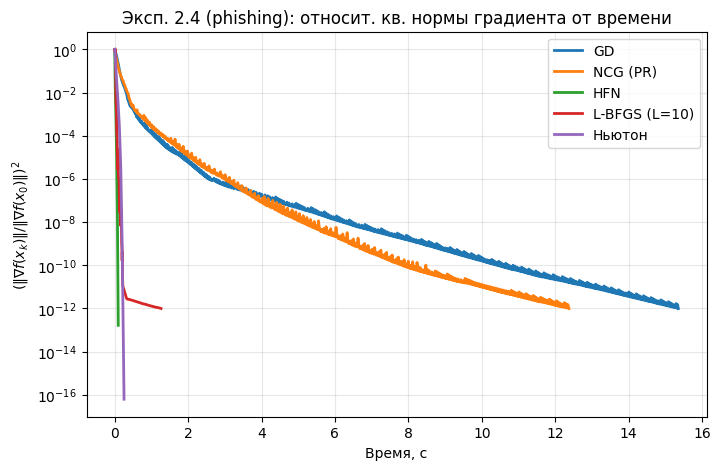
\includegraphics[width=\linewidth]{exp24_gradnorm_vs_time_phishing}\\
        \footnotesize 2.4: пример, phishing (градиент / время)
      \end{center}
    \end{column}
    \begin{column}{0.48\textwidth}
      \begin{center}
        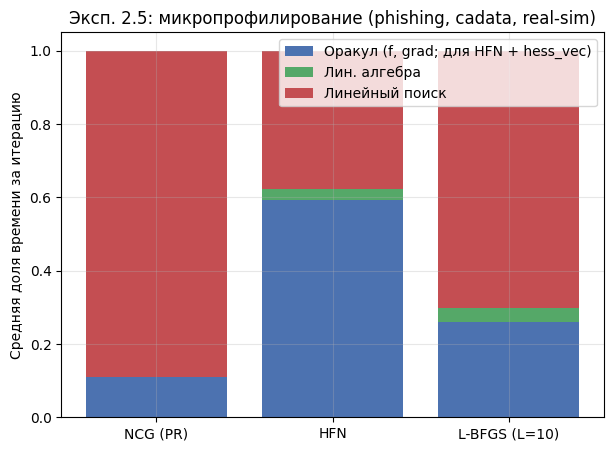
\includegraphics[width=\linewidth]{exp25_microprofiling}\\
        \footnotesize 2.5: микропрофилирование (NCG, HFN, L-BFGS)
      \end{center}
    \end{column}
  \end{columns}
\end{frame}

\begin{frame}{Эксперимент 2.6: обучение и обобщение}
  \begin{center}
    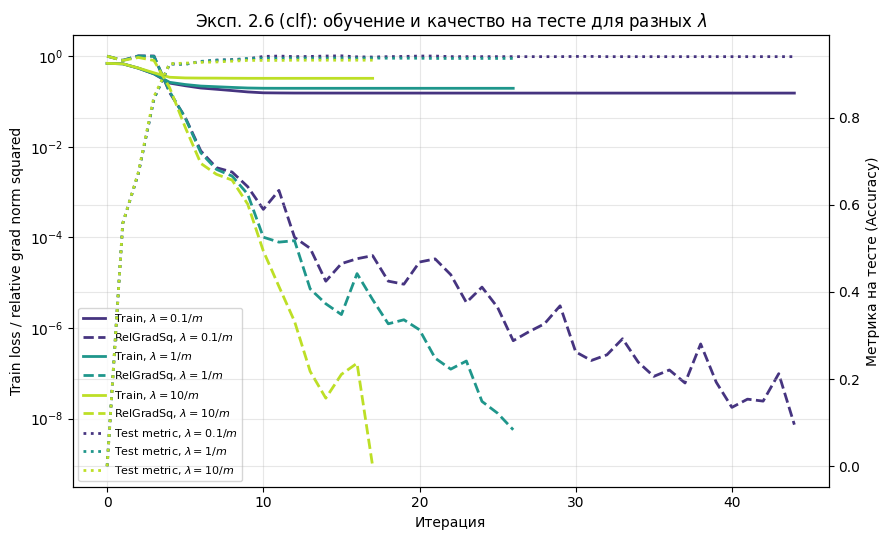
\includegraphics[height=0.72\textheight]{exp26_train_vs_quality_clf}
  \end{center}
  \vspace{-0.5em}
  {\footnotesize Аналогичный график для регрессии: \texttt{exp26\_train\_vs\_quality\_reg.png}.}
\end{frame}

\begin{frame}{Трек 4: вместо Вульфа — Cautious L-BFGS}
  \begin{itemize}
    \item Условие ``осторожного'' шага: $\displaystyle \frac{\langle s_k, y_k \rangle}{\lVert s_k \rVert^2} > \varepsilon \lVert \nabla f(x_k) \rVert^\alpha$.
    \item Ниже — сравнение по времени (ось $Y$ — относит.\ кв.\ нормы градиента) на \textit{phishing} после фиксации $x_0 \sim \mathcal{N}(0, 10)$.
  \end{itemize}
  \begin{center}
    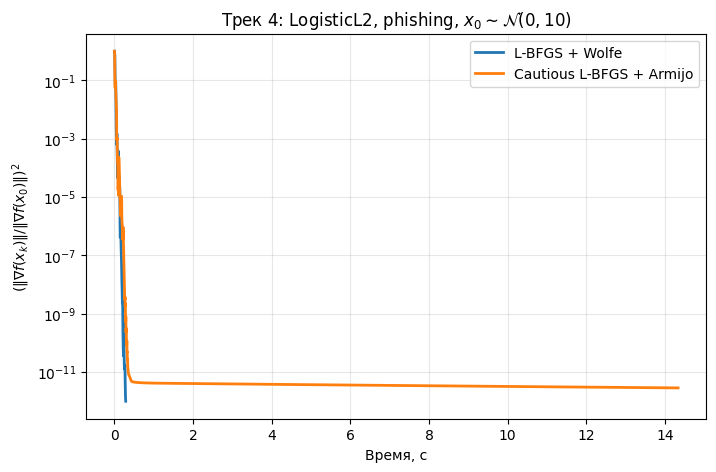
\includegraphics[width=0.72\linewidth]{track4_comparison_ml_phishing}
  \end{center}
\end{frame}

\begin{frame}{Выводы команды}
  \begin{itemize}
    \item % TODO: L-BFGS / HFN / время
    \item % TODO: микропрофилирование: где узкое место
    \item % TODO: 2.6: плато теста vs train
    \item % TODO: трек~4: Armijo + cautious vs Wolfe
  \end{itemize}
\end{frame}

\end{document}
